\cleartooddpage[\thispagestyle{empty}]
\chapter{Vortex Analysis to predict IA Initiation}\label{CHAPTER4}
The tangential, frictional stress caused by blood flowing along the vessel wall is known as WSS. The ANSYS-FLUENT software calculates WSS by the normal velocity gradient at the vessel wall:
	\begin{equation}
\tau\textsubscript{w} = \mu\frac{\partial v}{\partial n}
	\end{equation}
where $\mu$ is the dynamic viscosity. In this work, areas of high WSS were of interest as it is thought to play a role in the IA initiation \cite{Meng1254}. High WSS was defined as values $\ge$ 20 Pa during peak systole of the MRI waveform.

The WSSG was calculated using in-house VMTK scripts and is derived from three spatial derivatives of the WSS as follows:
	\begin{equation}
WSSG = \sqrt{(\frac{\partial{\tau_{w}}}{\partial{x}})^2 + (\frac{\partial{\tau_{w}}}{\partial{y}})^2 + (\frac{\partial{\tau_{w}}}{\partial{z}})^2}
	\end{equation}
with the time-averaged WSSG calculated as
	\begin{equation}
WSSG\textsubscript{av} = \frac{1}{T}\int_{0}^{T} | WSSG | dt
	\end{equation}
	
OSI is a nondimentional parameter, computing oscillations in the direction of the WSS vectors over the course of a cardiac cycle:
	\begin{equation}
OSI=\frac{1}{2}\left\{1-\frac{| \int_{0}^{T} \mathrm{\tau}_{i}dt |}{\int_{0}^{T} | \mathrm{\tau}_{i} | dt}\right\}
	\end{equation}
were $\tau\textsubscript{i}$ represents the WSS vector at a given time step across the duration of the cardiac cycle (T). The OSI describes the changes of a WSS vector's alignment with the cardiac cycle's temporally-averaged WSS vector. An OSI of 0 indicates no change in directionality and 0.5 being a complete direction reversal. 

The AFI \cite{Mantha1113} quantifies the variation in angle between the instantaneous WSS vector and time-averaged WSS vector:
	\begin{equation}
AFI=cos(\theta)=\frac{\mathrm{\tau}_{i}\cdot \mathrm{\tau}_{av}}{| \mathrm{\tau}_{i} |*| \mathrm{\tau}_{av}|}
	\end{equation}
For each point along the vessel wall, the minimum AFI calculated during the cardiac cycle was used to indicate the greatest deviation of the WSS vector from its mean direction. A minimum AFI of -1, 0, and 1 indicate deviations of 180\textdegree, 90\textdegree, and 0\textdegree respectively.

The GON index \cite{Shimogonya2009} quantifies fluctuations in WSSG directionality over the cardiac cycle. 
	\begin{equation}
GON=1-\frac{|\int_{0}^{T}Gdt|}{\int_{0}^{T}| G | dt}
	\end{equation}
T is the period of the cardiac cycle and G is the spatial wall shear stress gradient vector


The human vasculature is a system aimed at carrying blood and lymph through the body. The arteries of the vascular system help deliver oxygenated blood, nutrients, and components such as inflammatory markers and hormones through the body, while the veinous structures help take cellular and tissue waste matter to organs such as the lungs, liver and kidneys for removal as well as carrying deoxygentaed blood back to the heart. The lympahtic vessels carry lymph (fluid containing water and blood cells) to help maintain hemodynamic pressures withing the body. Intracranial aneurysms have only been shown to develop within the arterial portion of the vasculature, and as such will be the the part of the vascualture fouced upon in this work. The innermost layer of arteries, known as the tunica intima, is made of a monolayer of endothelial cells (EC) supported by a layer of collagen and elastin. This intimal layer comes into direct contact with the hemodynamic flow environment of the lumen (hollow cavity of the arterial system in which blood flows). This endothelial layer serves multiple purposes: hemodynamic mechanosensors, reacting to fluid forces and transducing said force into biochemical signals triggering cellular cascades controlling vascular tone and homeostasis\cite{dorland2017cell,cancel2016endothelial,chien2007mechanotransduction}, and acting as a selective permeability layer for macromolecules\cite{benn2016ve,ghim2017visualization,mundi2018endothelial}. Underlying the intima layer is the the tunica media, or media, a layer composed of smooth muscle cells, elastic connective tissue and collagen fibers. The main purpose of the media layer is to contract or dilate the arterial vasculature in response to (as signaled by the intima layer) differing hemodynamic conditions as a means to regulate circulation within the body\cite{bogunovic2019impaired,michel2018genetics}. The outermost layer of arteries, the tunica externa/adventitia, is composed of collagen fibers and elastic tissue helping to maintain the mechanical properties of the vasculature, while the collagen having a secondary purpose of anchoring the vessel to surrounding tissues (improving vessel stability)(Fig.~\ref{Vasculature_Layers}).

\begin{figure}[!h]
  \begin{center}
    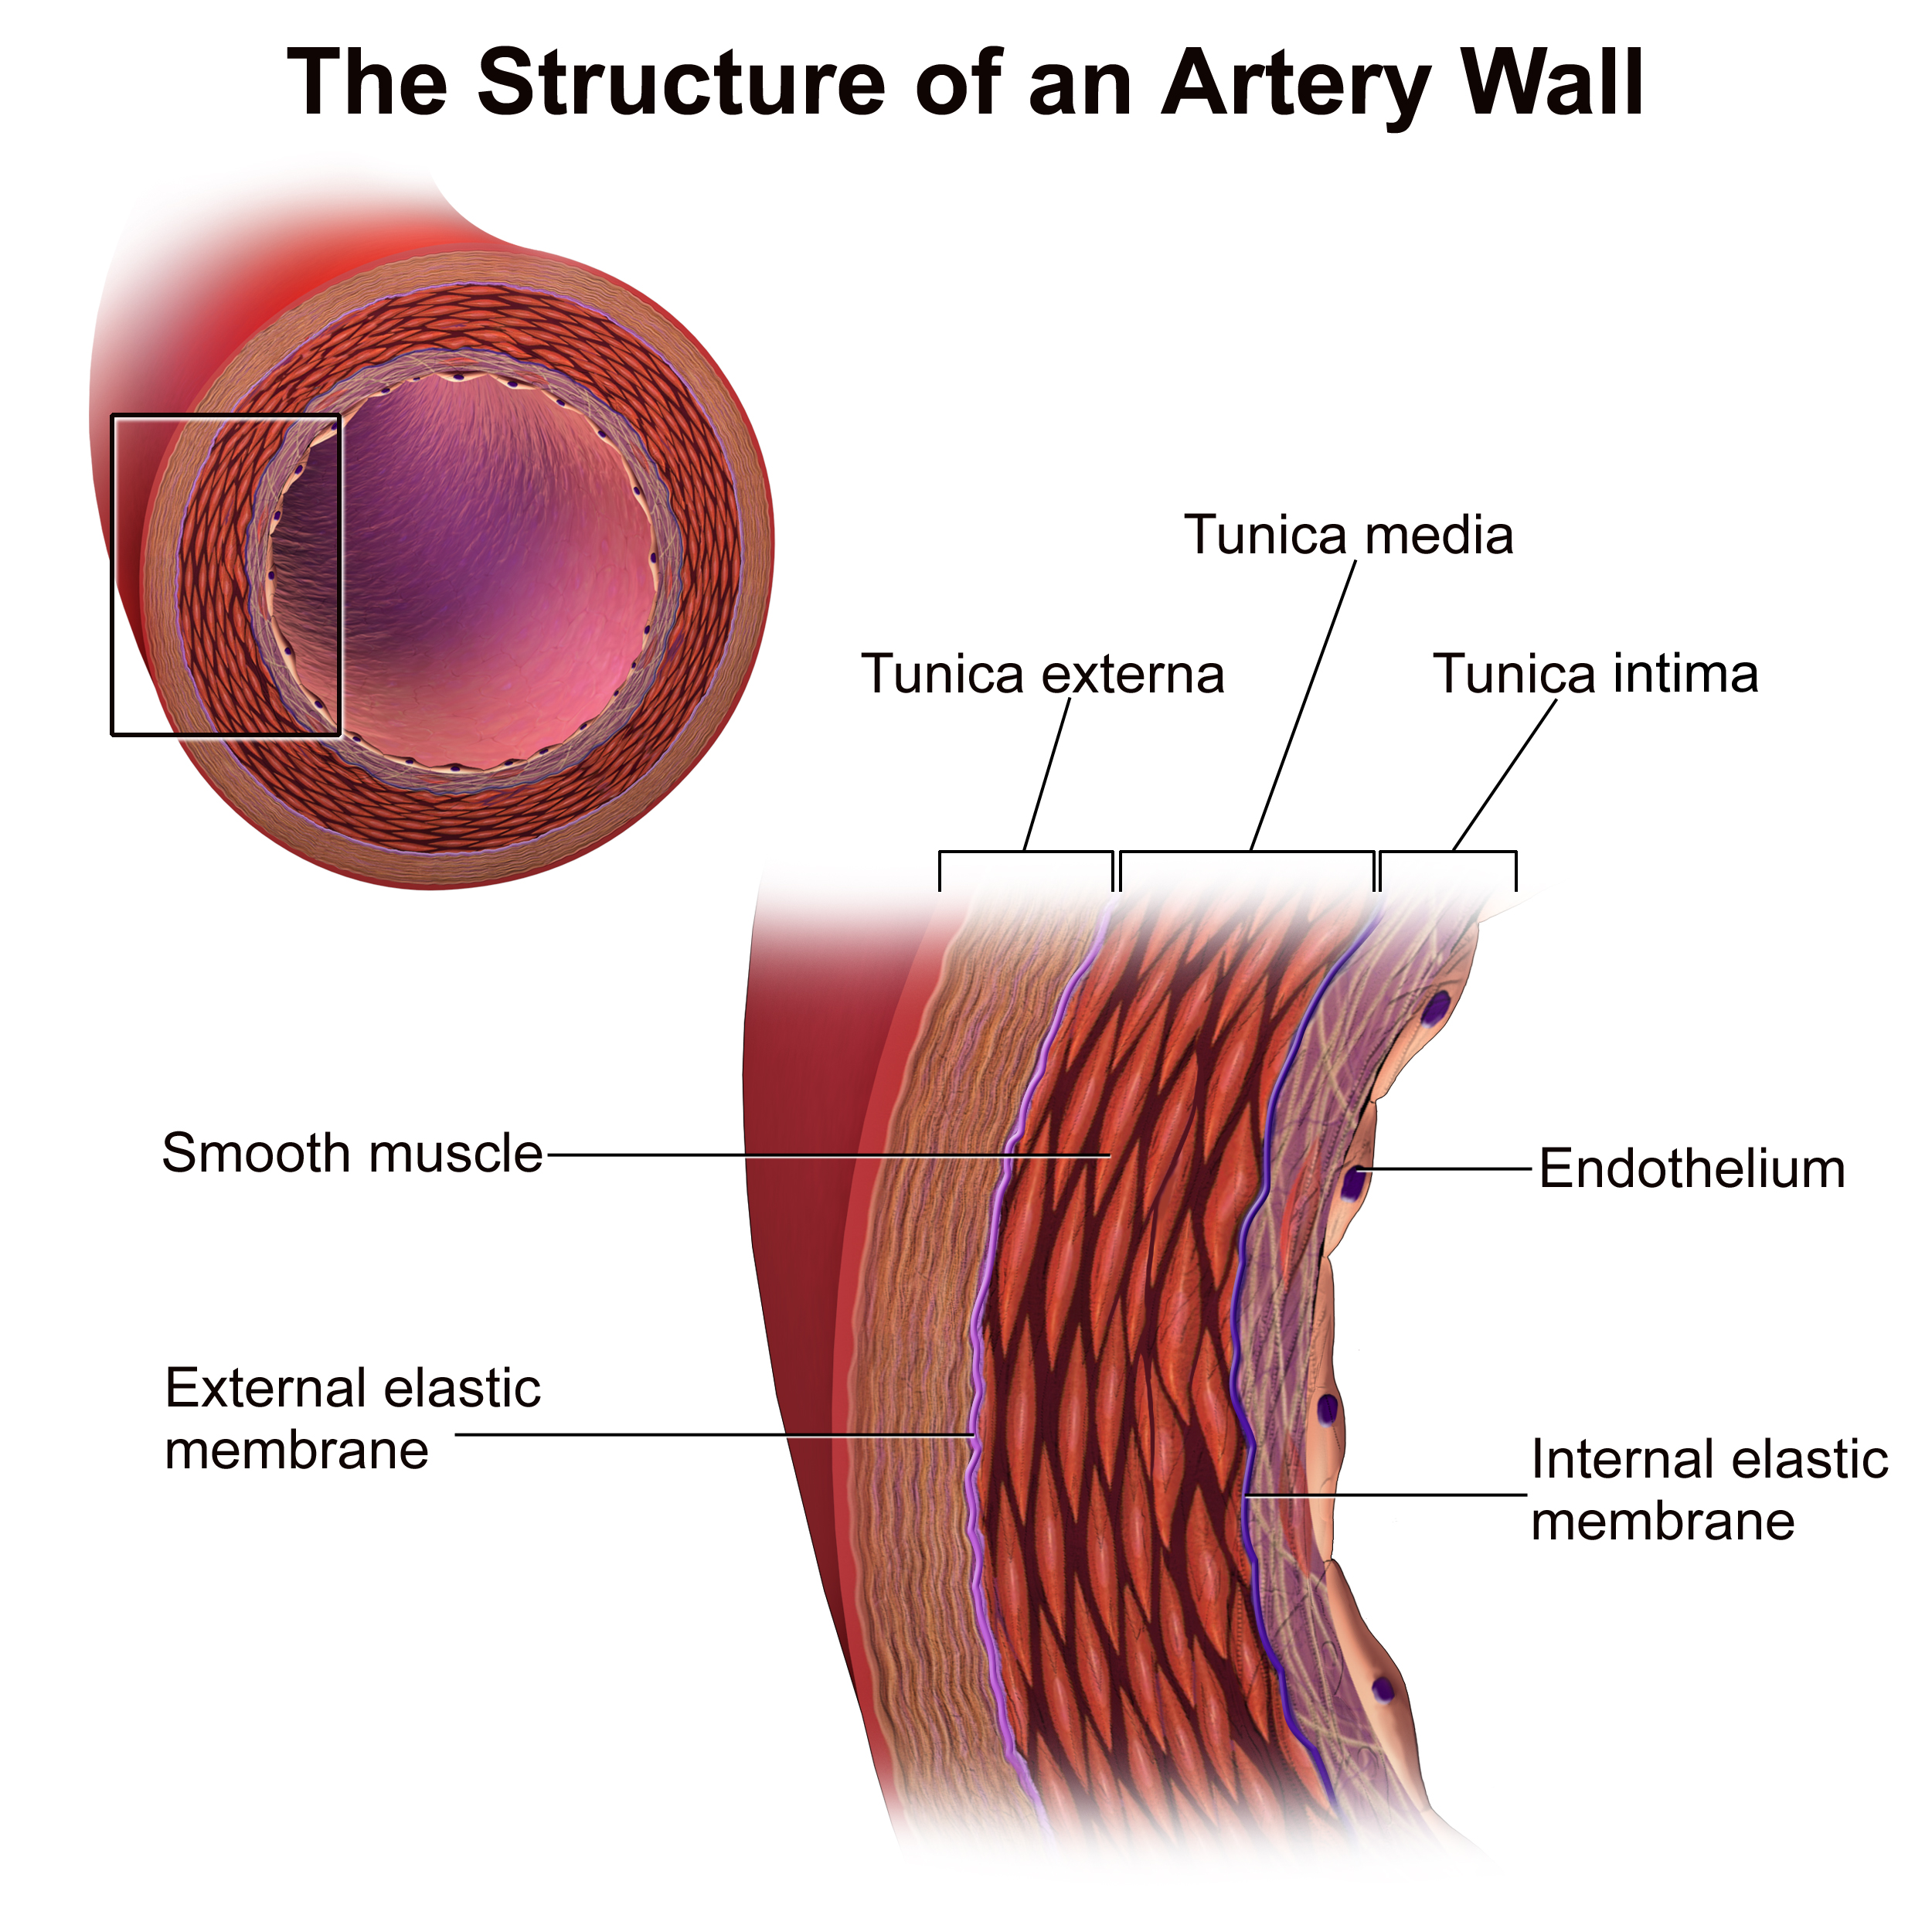
\includegraphics[width=3.5in]{Vasculature}
  \end{center}
  \caption{Layers of the vasculature. Original image from \cite{WIKI_Vessel}}
  \label{Vasculature_Layers}
\end{figure}